\documentclass[sigconf]{acmart}

\usepackage{booktabs} % For formal tables
\usepackage{amsmath}
\usepackage{amsfonts}
\usepackage{amssymb}
\usepackage{caption}
\usepackage{subcaption}
\usepackage{algorithm}
\usepackage{algpseudocode}


\begin{document}
\pretolerance=9999

\copyrightyear{2018}
\acmYear{2018}
\setcopyright{acmcopyright}
\acmConference[GECCO '18 Companion]{Genetic and Evolutionary Computation Conference Companion}{July 15--19, 2018}{Kyoto, Japan}
\acmBooktitle{GECCO '18 Companion: Genetic and Evolutionary Computation Conference Companion, July 15--19, 2018, Kyoto, Japan}
\acmPrice{15.00}
\acmDOI{10.1145/3205651.3208304}
\acmISBN{978-1-4503-5764-7/18/07}

\title[The Automated Design of Probabilistic Selection\\Methods for Evolutionary Algorithms]{The Automated Design of Probabilistic Selection Methods for Evolutionary Algorithms}

\author{Samuel N. Richter}
\affiliation{
  \institution{Missouri University of Science and Technology}
  \city{Rolla} 
  \state{Missouri} 
  \country{U. S. A.}
}
\email{snr359@mst.edu}

\author{Daniel R. Tauritz}
\affiliation{
  \institution{Missouri University of Science and Technology}
  \city{Rolla} 
  \state{Missouri} 
  \country{U. S. A.}
}
\email{dtauritz@acm.org}

\begin{abstract}
Selection functions enable Evolutionary Algorithms (EAs) to apply selection pressure to a population of individuals, by regulating the probability that an individual's genes survive, typically based on fitness. Various conventional fitness based selection methods exist, each providing a unique relationship between the fitnesses of individuals in a population and their chances of selection. 
However, the full space of selection algorithms is only limited by max algorithm size, and each possible selection algorithm is optimal for some EA configuration applied to a particular problem class. Therefore, improved performance may be expected by tuning an EA's selection algorithm to the problem at hand, rather than employing a conventional selection method. The objective of this paper is to investigate the extent to which performance can be improved by tuning selection algorithms, employing a Hyper-heuristic to explore the space of search algorithms which encode the relationships between the fitnesses of individuals and their probability of selection. We show the improved performance obtained versus conventional selection functions on fixed instances from a benchmark problem class, including separate testing instances to show generalization of the improved performance.
\end{abstract}


\begin{CCSXML}
<ccs2012>
<concept>
<concept_id>10010147.10010257.10010293.10011809.10011813</concept_id>
<concept_desc>Computing methodologies~Genetic programming</concept_desc>
<concept_significance>500</concept_significance>
</concept>
<concept>
<concept_id>10003752.10003809</concept_id>
<concept_desc>Theory of computation~Design and analysis of algorithms</concept_desc>
<concept_significance>300</concept_significance>
</concept>
<concept>
<concept_id>10011007.10011074.10011092.10011782.10011813</concept_id>
<concept_desc>Software and its engineering~Genetic programming</concept_desc>
<concept_significance>300</concept_significance>
</concept>
</ccs2012>
\end{CCSXML}

\ccsdesc[500]{Computing methodologies~Genetic programming}
\ccsdesc[300]{Theory of computation~Design and analysis of algorithms}
\ccsdesc[300]{Software and its engineering~Genetic programming}


\keywords{Selection, Genetic Programming, Hyper-heuristic}

\maketitle

\section{Introduction}
\label{Introduction}

Evolutionary Algorithms employ selection functions to control the probability that an individual's genes are selected for recombination and survival. Various conventional fitness-based selection methods exist, each providing a unique relationship between the fitness of individuals in a population and their chances of selection. Because of this, each selection algorithm plays a significant role in determining the selective pressure of the EA, and thus, the average performance of the EA's search through the space of solutions~\cite{woodward2010metaBias}. Many selection algorithms are parameterized, allowing for further variance in the selective pressure they provide. In cases where parameterized selection algorithms are applied, the parameters can be carefully tuned, either manually or with tuning software, to maximize the performance of an EA on a particular problem or problem class.

New selection algorithms can be designed in cases where the performance offered by existing algorithms is insufficient, even with well-tuned parameters. However, the full space of selection algorithms is only limited by the maximum algorithm size, and so it is highly unlikely that any designed algorithm offers the optimal selection behavior for the EA. According to the "No Free Lunch" theorem, each possible selection algorithm is optimal for some EA configuration applied to a particular problem class~\cite{wolpert1995noFreeLunch}. Therefore, a performance gain can be expected from exploring the space of selection algorithms to find one that offers better performance than any previously considered. Previous work has confirmed this hypothesis, prompting our approach to use a Hyper-heuristic and a custom representation of selection functions to explore the space of new selection functions ~\cite{woodward2011selection}.

Our approach employs a Hyper-heuristic to explore the space of selection algorithms, with each search algorithm represented by a binary Koza-style GP-tree~\cite{koza1994genetic}. Each tree controls the probability that an individual will be selected for recombination, as a mathematical function with various terminal values, including the individual's fitness, fitness ranking in the population, and the size of the population.

The rest of this paper is organized as follows: Section~\ref{Background} gives an overview of previous work related to this subject matter, including an overview of Hyper-heuristics, automated algorithm design, and the targeted improvement of Evolutionary Algorithm Components. Section~\ref{Methodology} describes our methodology for encoding selection functions and searching through the space of selection functions. Section~\ref{Experimental Setup} describes the setup and parameters used in our experiment. Section~\ref{Results} shows our results, which we analyze and discuss in Section~\ref{Discussion}. We then summarize our experiment and state our conclusions in Section~\ref{Conclusion} and discuss avenues for future work on this subject in Section~\ref{Future Work}.

\section{Background}
\label{Background}
The field of Hyper-heuristics encompasses many different approaches for the evolution of new algorithms. Methods may utilize offline learning, in which computation is done \textit{a prioiri} to develop a heuristic, or online learning, in which a heuristic is developed dynamically alongside a running problem. Hyper-heuristic searches can be perturbative, in which complete solutions are considered individually, or constructive, in which solutions begin partially built and are extended iteratively~\cite{burke2013HHstateoftheart}.

A major application of Hyper-heuristics is the automated design of algorithmic components, which various algorithms have been shown to benefit from. Hyper-heuristics have been used to evolve new algorithms from components of existing algorithms for Ant Colony optimization algorithms, Boolean Satisfiability solvers, local search heuristics, and iterative parse trees representing Black Box Search Algorithms~\cite{lopez2012antcol, khudabukhsh2009satenstein, martin2013evolvingBBSA, burke2012localHeuristics}. This experiment applies the same concept to selection functions, using Hyper-heuristics to build selection functions from smaller components to search the space of new selection functions.

There is also published work on improvement of targeted components of EAs, including the evolution of new mutation operators, mating preferences, genetic representation of individuals, and crossover operators~\cite{woodward2012mutationGeneration, guntly2011limp, goldman2011scc, scott2015geneticRepresentations, hong2013probMutation}. Methods for generating selection algorithms, in particular, have been investigated. A random walk through the space of register machines that compute and return a probability of selection for each individual showed that such custom-tuned selection algorithms can outperform typical selection algorithms~\cite{woodward2011selection}. In the previous work involving the evolution of Black Box Search Algorithms, the parse trees include evolved selection functions, although the selection functions are limited to two conventional selection functions (\textit{k}-tournament and truncation) with evolved parameters. An evolutionary search through selection functions developed with Grammatical Evolution showed that better selection functions can be developed using a Hyper-heuristic, and that the performance of these selection functions can generalize to new instances within the same problem class~\cite{lourencco2013selection}. The work described in this paper expands on these ideas with a new representation for selection algorithms: an encoding of the relationship between an individual's fitness and its probability of selection for recombination within a Koza-style GP-Tree. 

\section{Methodology}
\label{Methodology}

Here we discuss the methodology of our meta-EA. We outline the format we use to represent selection strategies in the meta-EA, and show how typical selection strategies, such as fitness-proportional and \textit{k}-tournament, would be represented in this format. We then discuss how we will use the meta-EA to evaluate and search for new selection strategies.

\subsection{Encoding Selection Functions}
\label{Methodology-Encoding Selection Functions}

Most typical selection functions are formatted as a series of algorithmic steps to perform on a population of individuals, that ultimately returns the selected individual(s). While we could explore the entire combinatorial space of algorithmic steps to find new selection functions, doing so could generate many algorithms which are not valid selection functions, or even functional algorithms. Therefore, we need a representation of selection functions that is both robust enough to represent a wide variety of selection functions, yet restrained enough that we can effectively search within it to find new, valid selection algorithms.

We represent selection functions as binary Koza-style GP-trees~\cite{koza1994genetic}, with one tree representing one selection function. Rather than encoding entire programs within the GP-Tree, which could result in an infeasably wide search space of selection algorithms, the GP-Trees instead encode mathematical functions ~\cite{woodward2009GPNotGood}. To perform selection on a population, the function is evaluated once for each member of the population. The output values are normalized to positive values if any of them are negative, then a weighted random selection is performed, using the values as weights for each corresponding individual in the population. This method is very similar to fitness proportional selection, but instead of using the fitness of each individual as its proportional chance to be selected, the output of a mathematical function encoded in a GP-tree is used. The terminals of the GP-tree, and thus the inputs to the function, include the individual's fitness, the individual's fitness ranking among the population members, the total size of the population, constants, and random terminals, which return a random number within a closed range. Binary operators in the GP-Tree include mathematical functions (+, -, *, /) and the step function, which takes two inputs and returns 1 when the first input is greater than the second, and 0 otherwise. The GP-tree also includes a single bit that determines whether the selection is performed with or without replacement. If the bit is disabled, then the GP-Tree will not select the same individual twice within the same generation.

An example of this representation is shown in Figure~\ref{fig:example_adpsea}. The figure shows an example of the GP-Tree that represents the function evaluated for each individual, as well as the status of the bit determining whether selection is performed with replacement. The psuedocode for this method of selection is shown in Algorithm \ref{alg:ExampleSelection}. Note the \textproc{WeightedSelection} procedure, which is the final step in all selection functions of this representation, which takes the output weights provided by the GP-Tree, normalizes them if necessary, and then performes a weighted selection. Also note the code at line \ref{line:SelectWithoutReplacementLine}, which removes selected individuals from the candidate pool if selection is being performed without replacement. This line is omitted in strategies that select with replacement.

Figure ~\ref{fig:selection_chances} shows how, for a hypothetical sample population of nine individuals, different selection functions will result in different probabilities of each individual being selected. The graph also includes the selection probabilities for the custom selection algorithm represented by the GP-Tree in Figure~\ref{fig:example_adpsea}. This graph visualizes the notion that the probability of an individual being selected is a direct function of the selection method used, and that new selection methods can provide new distributions for probability of selection over the population. 

\begin{figure}
    \centering
    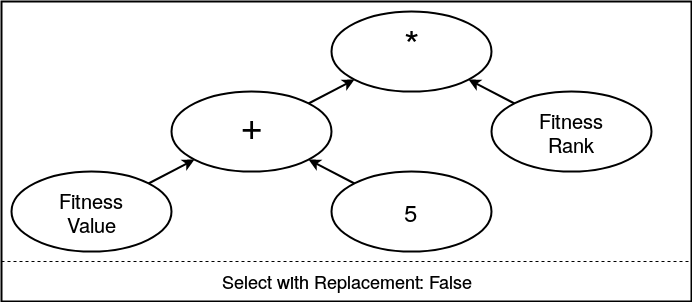
\includegraphics[width=0.475\textwidth]{example_adpsea}
    \caption{Example of a generated selection function, encoded in a GP-Tree. With this selection function, the probability of any individual being selected is directly proportional to the individual's fitness rating plus 5, multiplied by the individual's ranking in the population ordered by fitness. The bit to indicate selection with replacement is set to False, so this selection function will not select the same individual more than once within the same generation.}
    \label{fig:example_adpsea}
\end{figure}

\begin{algorithm}
\caption{Probabilistic Selection Function}
\label{alg:ExampleSelection}
\begin{algorithmic}[1]
\Procedure {WeightedSelection}{$P$, $W$} \label{proc:WeightedSelection}
	\State $w_{min} \leftarrow minimum(W)$	
	\State $s \leftarrow 0$
	\ForAll {$w \in W$}
		\If {$w_{min}  < 0$}
			\State $s \leftarrow s + (w - w_{min} )$			
		\Else
			\State $s \leftarrow s + w$		
		\EndIf	
	\EndFor
	\State{$r \leftarrow random(0,s)$}
	\State $i \leftarrow 1$
	\While {$r > W(i)$}
		\State $r \leftarrow r + W(i)$
		\State $i \leftarrow i + 1$
	\EndWhile	
	\State \textbf{return} $P(i)$
\EndProcedure
\Statex
\Procedure {ExampleSelection}{$P, replace$}
	\For {$i \leftarrow 1,n$}
		\State $W(i) \leftarrow (P(i).Fitness+5) \cdot P(i).FitnessRank$
	\EndFor
	\State $selected \leftarrow \Call{WeightedSelection}{P, W}$
	\State \textbf{remove} $selected$ \textbf{from} $P$ \label{line:SelectWithoutReplacementLine}
	\State \textbf{return} $selected$
\EndProcedure
\end{algorithmic}
\end{algorithm}

\begin{figure}
    \centering
    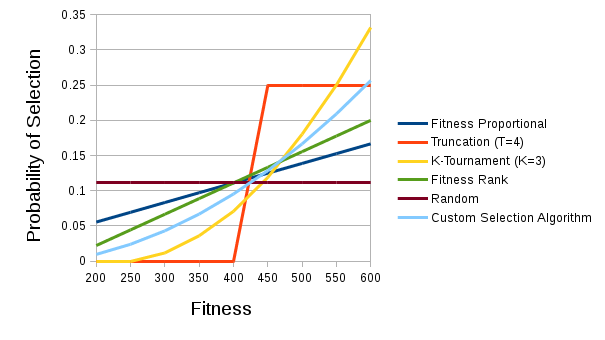
\includegraphics[width=0.475\textwidth]{selection_chances}
    \caption{A comparison of the chances that each member of a sample population, with fitnesses as listed, will be selected, under each of the typical selection strategies listed, as well as the custom selection strategy shown in Figure~\ref{fig:example_adpsea}.}
    \label{fig:selection_chances}
\end{figure}

\subsection{Representing Typical Selection Functions}
\label{Methodology-Representing Typical Selection Functions}

In order to be able to make a fair comparison between selection algorithms encoded in this representation and the selection algorithms typically used in Evolutionary Algorithms, we must show that such typical selection algorithms can be encoded in this representation. Thus, we must find GP-Trees which have the same probability of selecting individuals in the population as the typical selection functions in their standard, algorithmic form.

The probability $P_i$ of an individual $i$ being selected by a selection function encoded by a GP-Tree is given as

\begin{equation}
  P_i =
  \begin{cases}
    R_i / \sum_{j=1}^n R_j & \text{if $R_{min}\geq0$} \\
    (R_i - R_{min}) / \sum_{j=1}^n (R_j - R_{min}) & \text{if $R_{min}<0$} \\
  \end{cases}
\end{equation}
\\

\noindent where $R_i$ is the relative selection probability of individual $i$, output by the function encoded in the GP-Tree, $R_{min}$ is the minimum value $R$ output for the current population, and $n$ is the size of the pool of candidates available for selection. If the GP-Tree does not select with replacement, then the population member is removed from the selection pool after it is selected, and the probability of selection is recalculated for the remaining individuals.

The simplest selection function to represent with the GP-Tree is fitness proportional selection. In fitness proportional selection, the fitness of the individual is directly used as the relative probability of selection, so the GP-Tree only needs to include the \textit{fitness} terminal value as its single node, and $R_i$ is calculated as follows:
\begin{equation}
	R_i = fitness_i
\end{equation}
where $fitness_i$ is the fitness of individual $i$. Similarly, fitness-ranking selection ranks the individuals in the population from greatest to least fitness, and uses each individual's fitness ranking as the relative probability of selection. Because the fitness-ranking is also a simple terminal value in the GP-Tree, $R_i$ can be calculated as follows:
\begin{equation}
	R_i = fitnessRank_i
\end{equation}
where $fitnessRank_i$ is the fitness ranking of individual $i$. In both cases, the GP-Tree will select with replacement, so an individual may be selected more than once.

In truncation selection, the top $N$ individuals are selected, where $N$ is exactly the number of individuals who must be selected (typically twice the number of children to be produced, if each child requires two parents to produce it). To represent this function, we must have a GP-Tree that assigns a non-zero relative probability of selection to the top N individuals in the population, and a zero relative probability of selection to all others. This can be described as follows:
 
\begin{equation}
  R_i =
  \begin{cases}
    1 & \text{if $fitnessRank_i > popSize-N$} \\
    0 & \text{$otherwise$} \\
  \end{cases}
\end{equation}
\\

\noindent where $popSize$ is the size of the population. This stepwise behavior can be achieved by the GP-Tree with the \textit{step} operator, which returns 1 if the left operand is greater than or equal to the right operand, and 0 otherwise. Such a GP-Tree will effectively select individuals at random from the top $N$ individuals, since each of those individuals is assigned the same relative probability of selection. However, if the GP-Tree does not select with replacement, then each individual can only be selected once, and since the GP-Tree will select $N$ individuals, it will select all of the top $N$ individuals.

Modeling \textit{k}-tournament selection with a GP-Tree is less straightforward. To be selected by \textit{k}-tournament selection, an individual must both be selected to be in a tournament, and have the highest fitness of all individuals in that tournament. Thus, the probability that an individual is selected by \textit{k}-tournament selection is equal to the probability of being selected for a tournament, times the probability of winning the tournament:
\begin{equation}
\begin{aligned}
	P_i = P(individual\ i\ selected\ for\ tournament)\\ \cdot P(individual\ i\ wins\ tournament)
\end{aligned}
\end{equation}

The probability of being selected for a tournament is simply the size of the tournament $k$ divided by the population size: 
\begin{equation} \label{eq:probabilitySelectedForTournament}
	P(individual\ i\ selected\ for\ tournament) = k / popSize
\end{equation}

To win a tournament, every other individual in the tournament must have a fitness rank less than the to-be winner's fitness rank. This can be modeled as another product of probabilities:
\begin{equation} 
\begin{aligned}
	P(individual\ i\ wins\ tournament) =\\ \prod_{j=1}^{k-1} P(fitnessRank_j < fitnessRank_i)
\end{aligned}
\end{equation}

The probability that individual $j$ has a lower fitness rank than individual $i$ can be calculated as a function of the population size and $fitnessRank_i$, with subtractions to account for the fact that individuals cannot be chosen twice for the same tournament. This probability is as follows:

\begin{equation} \label{eq:probabilityWinTournament}
\begin{split}
	P(individual\ i\ wins\ tournament) =\\ {k / n} \cdot \prod_{j=1}^{k-1} \frac{fitnessRank_i - j}{n - j}
\end{split}
\end{equation}

Thus, the full probability that an individual is selected by \textit{k}-tournament is the product of equations \ref{eq:probabilitySelectedForTournament} and \ref{eq:probabilityWinTournament}. Because this probability sums to 1, and is positive for every individual i the population, no normalization step is necessary, and so $R_i = P_i$. Thus, the full relative probability of selection $R_i$ for \textit{k}-tournament can be calculated as follows:

\begin{equation}
	R_i = P_i = {k / popSize} \cdot \prod_{j=1}^{k-1} \frac{fitnessRank_i - j}{n - j}
\end{equation}
\\

This formula can be expanded into a form that uses only the basic mathematical functions and the terminals used by the GP-Tree, and so we can represent \textit{k}-tournament selection using our GP-Tree representation.

Example GP-Trees encoding the selection functions discussed here are displayed in Figure~\ref{fig:example_selections}. The psuedocode for the selection strategies represented by these GP-Trees is shown in Algorithms \ref{alg:FitnessProportionalSelection}, \ref{alg:FitnessRankingSelection}, \ref{alg:TruncationSelection}, and \ref{alg:KTournamentSelection}.

\begin{figure*}
    \centering
    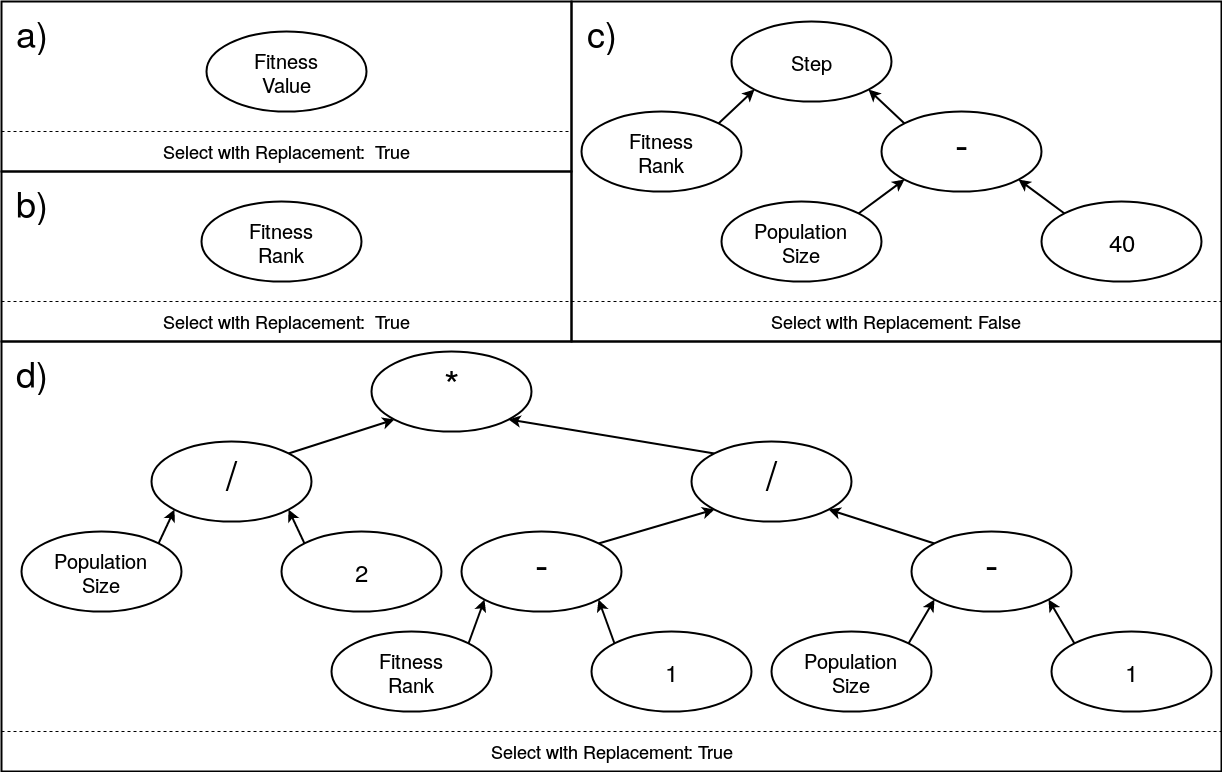
\includegraphics[width=0.9\textwidth]{example_selections}
    \caption{The GP-Trees encoding the selection probabilities for typical selection functions, including a) Fitness proportional, b) Fitness Ranking, c) Truncation (T=40), and d) \textit{k}-tournament (k=2).}
    \label{fig:example_selections}
\end{figure*}

\begin{algorithm}
\caption{Fitness Proportional Selection}
\label{alg:FitnessProportionalSelection}
\begin{algorithmic}[1]
\Procedure {FitnessProportionalSelection}{$P$}
	\For {$i \leftarrow 1,n$}
		\State $W(i) \leftarrow P(i).Fitness$
	\EndFor
	\State $selected \leftarrow \Call{WeightedSelection}{P, W}$	
	\State \textbf{return} $selected$
\EndProcedure

\end{algorithmic}
\end{algorithm}

\begin{algorithm}
\caption{Fitness Ranking Selection}
\label{alg:FitnessRankingSelection}
\begin{algorithmic}[1]
\Procedure {FitnessRankingSelection}{$P$}
	\For {$i \leftarrow 1,n$}
		\State $W(i) \leftarrow P(i).FitnessRank$
	\EndFor
	\State $selected \leftarrow \Call{WeightedSelection}{P, W}$	
	\State \textbf{return} $selected$
\EndProcedure
\end{algorithmic}
\end{algorithm}

\begin{algorithm}
\caption{Truncation Selection}
\label{alg:TruncationSelection}
\begin{algorithmic}[1]
\Procedure {TruncationSelection}{$P, t$}
	\For {$i \leftarrow 1,n$}
		\If {$P(i).FitnessRank > t$}
			\State $W(i) \leftarrow 1$
		\Else
			\State $W(i) \leftarrow 0$
		\EndIf
	\EndFor
	\State $selected \leftarrow \Call{WeightedSelection}{P, W}$
	\State \textbf{remove} $selected$ \textbf{from} $P$	
	\State \textbf{return} $selected$
\EndProcedure
\end{algorithmic}
\end{algorithm}

\begin{algorithm}
\caption{\textit{k}-tournament Selection}
\label{alg:KTournamentSelection}
\begin{algorithmic}[1]
\Procedure {KTournamentSelection}{$P, k$}
	\For {$i \leftarrow 1,n$}
		\State $W(i) \leftarrow k/n$
		\For {$j \leftarrow 1, k-1$}
			\State $W(i) \leftarrow W(i) \cdot (P(i).FitnessRank - j)/(n-j)$
		\EndFor
	\EndFor
	\State $selected \leftarrow \Call{WeightedSelection}{P, W}$	
	\State \textbf{return} $selected$
\EndProcedure
\end{algorithmic}
\end{algorithm}

\subsection{Search Methodology}
\label{Methodology-Search Methodology}

We use a meta-EA to explore the space of selection functions by evolving the GP-trees described in Section~\ref{Methodology-Encoding Selection Functions}. The quality of each selection function is determined by running an underlying EA on a suite of static training instances from a benchmark problem class. All parameters of the bottom-level EA are kept constant, aside from the parent selection strategy. Each run of the bottom-level EA is terminated when the fitness of the population converges. The best fitness achieved in the final population of the underlying EA is used as a measure of the EA's performance, and the average performance of all runs of an EA using a particular selection function is used as the fitness of that selection function in the meta-EA.

When the meta-EA concludes, the bottom-level EA utilizing the best selection function from the meta-EA is run on a set of separate testing instances from the same problem class to test the generalization of the selection function's performance. For comparison, the same EA is run with a suite of typical selection functions, including fitness-proportional, fitness-ranking, \textit{k}-tournament (using several values for k), and truncation selection.

The benchmark problem class used for the underlying EA is the NK-Landscape class of problems.~\cite{kaufmann1993origins}. This benchmark was chosen because the properties of the fitness landscape can be easily controlled with the N and K parameters, as well as the policy with which the fitness values of the loci are generated. With one set of parameters, a wide range of new NK-Landscapes can be easily generated, making it easy to provide both a variety of training landscapes to tune a selection algorithm to, and a variety of new, separate landscapes to use for testing the generalization of the selection algorithm. 


\section{Experimental Setup}
\label{Experimental Setup}

\begin{table}
  \caption{Meta-EA Parameters}
  \label{tab:meta-EA_params}
  \begin{tabular}{cc}
    \toprule
    Parameter& Value\\
    \midrule
    Population Size & 50 \\
    Offspring Size & 50\\
    Evaluation Count & 2500\\
    Max GP-Tree Initialization Depth & 3\\
    Parent Selection & \textit{k}-tournament, \textit{k}=10 \\
    Survival Selection & Random\\
    Mutation & Subtree Regeneration\\
    Crossover & Subtree Crossover\\
    Parsimony Pressure Coefficient & 1\\
    Mutation Rate & 0.1\\
    Training Instances & 20 \\
    Runs per Training Instance & 3 \\
    Testing Instances & 50 \\
    Runs per Testing Instance & 100 \\
    Range for Constant Terminals & [-100, 100]\\
    Range for Random Terminals & [-100, 100]\\
    
  \bottomrule
\end{tabular}
\end{table}

Table ~\ref{tab:meta-EA_params} shows the parameters used in the meta-EA, which were selected with manual tuning to ensure the best performance of the meta-EA. 

Table ~\ref{tab:basicEA_params} shows the parameters used for each run of the bottom-level EA and the benchmark function. The benchmark parameters were selected to ensure that each benchmark problem was difficult enough to warrant the use of an EA, while not being so difficult that the meta-EA would quickly trend toward attractive but low-quality selection functions, such as aggressive hill-climbers. The bottom-level EA parameters were chosen so that the performance of the EA would vary heavily with the selection function used, so that high-quality selection functions could be easily exposed by the bottom-level EA.

For the bottom-level EA, the parent selection is performed by the evolved selection function, and random selection is used for survival selection. Because the survival selection is random, the selection pressure must be supplied by parent selection in order for the EA to be effective, to encourage the evolution of good selection strategies at the meta-EA level.

When generating the NK-Landscape training and testing instances, the values for N (genome length) and K (locus length) are kept constant. To generate each landscape, the locus epistatis is randomized, and each locus is assigned a random fitness value, selecting an integer between 0 and the locus length. Randomizing these two components for every instance of the benchmark problem leads to a wide variety of fitness landscapes for training and testing instances.

\begin{table}
  \caption{Bottom-level EA/Benchmark Function Parameters}
  \label{tab:basicEA_params}
  \begin{tabular}{cc}
    \toprule
    Parameter & Value\\
    \midrule
    Population Size & 100 \\
    Offspring Size & 20\\
    Genome Length (N) & 40 \\
    Locus Length (K) & 8\\
    Locus Minimum Value & 0\\
    Locus Maximum Value & 8\\
    Survival Selection & Random \\
    Termination Criteria & Convergence \\
    Generations to Convergence & 25\\
    Mutation & Random Bit Flip \\
    Mutation Rate & 0.05\\
    Crossover & Per-Bit Crossover\\
	
  \bottomrule
\end{tabular}
\end{table}

\section{Results}
\label{Results}

After running the meta-EA, a bottom-level EA using the best selection function was run against each of the 50 testing instances for 100 runs each. The GP-Tree representation of this selection function is shown in Figure~\ref{fig:adpsea_final}. The bottom level-EA is run on the same testing instances with a suite of typical selection functions, and the results are compared to the performance of the EA using the custom selection function. A two-sided t-test is run on the final best fitnesses achieved by the EA using the custom selection function versus the final best fitnesses achieved when using each of the typical functions. 

For 46 of the 50 testing instances, the EA using the custom selection functions significantly outperformed each EA using a typical selection function, with significance P<0.001 in all cases. For the remaining 4 testing instances, there was one selection function in the suite of typical selection functions whose performance was not significantly different from the custom selection function; the custom selection function outperformed all other typical selection functions in these 4 cases. 

Table ~\ref{tab:results} shows the final best fitness achieved by the underlying EA on the first 5 testing instances, using a number of conventional selection functions and the best custom-tuned selection function found by the meta-EA, to give a general idea of the performance achieved by the custom selection function on the testing instances. For these 5 testing instances, all differences between the performance of the custom selection algorithm and the performance of the typical selection algorithms are statistically significant, with P<0.001.

Figure~\ref{fig:nk_landscape_fitness_plot} shows the average performance over time of an EA using the best evolved selection functions on one testing instance, compared to the performance of the same EA using typical selection functions. Similar results were observed on the other testing instances. Figure~\ref{fig:nk_landscape_fitness_boxplot} shows a boxplot comparing the final best fitness values achieved on all of the runs on the same testing instances by the EA using the best evolved selection function and the typical selection functions.

\begin{table*}
  \caption{Final best fitness achieved by bottom-level EA on each testing instance, averaged over all runs, for the first 5 test instances.}
  \label{tab:results}
  \begin{tabular}{cccccc}
    \toprule
    Test Instance &1&2&3&4&5\\
    \midrule
    Custom Selection Function & 225.18 & 220.03 & 208.78 & 207.39 & 218.49 \\
	\textit{k}-tournament (\textit{k}=2) & 187.52  & 186.48 & 175.94 & 165.3 & 186.0 \\
	\textit{k}-tournament (\textit{k}=3) & 193.11 & 191.57 & 177.86 & 168.32 & 189.39 \\
	\textit{k}-tournament (\textit{k}=5) & 211.18 & 199.46 & 186.71 & 183.52 & 197.57 \\
	Fitness Proportional & 182.73 & 183.99 & 171.4 & 162.17 & 183.47 \\
	Fitness Ranking & 187.9 & 187.02 & 174.98 & 164.23 & 185.88 \\
	Truncation & 204.22 & 192.56 & 180.07 & 171.63 & 191.63 \\

  \bottomrule
\end{tabular}
\end{table*}

\begin{figure}
    \centering
    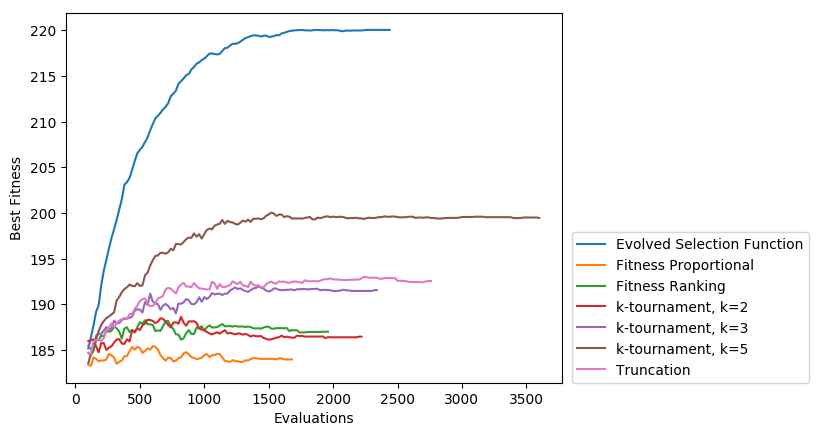
\includegraphics[width=0.478\textwidth]{nk_landscape_fitness_plot}
    \caption{The best fitness achieved by the underlying EA on one of the testing functions, using evolved and conventional fitness functions, averaged over all runs.}
    \label{fig:nk_landscape_fitness_plot}
\end{figure}

\begin{figure}
    \centering
    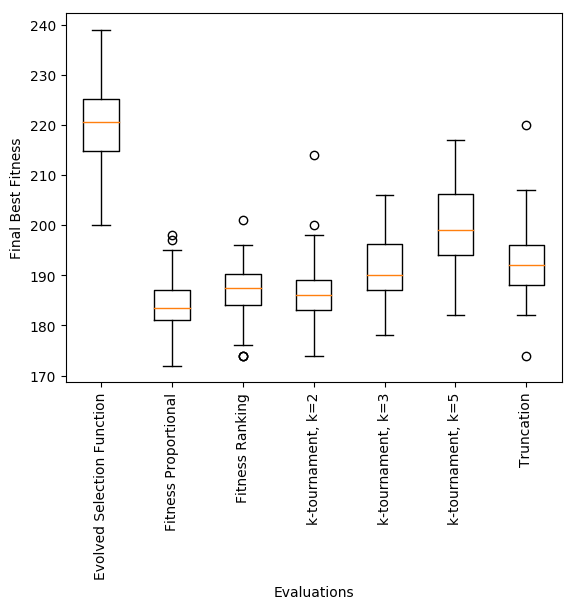
\includegraphics[width=0.475\textwidth]{nk_landscape_boxplot}
    \caption{A boxplot of the final best fitness values achieved by the underlying EA on one of the testing functions, using evolved and conventional fitness functions. Here, each box encloses the data points within the first and third quartiles, and the whiskers enclose the furthest data points that still lie within 1.5 *\textit{IQR} from each quartile, where textit{IQR} is the interquartile range.}
    \label{fig:nk_landscape_fitness_boxplot}
\end{figure}

\begin{figure}
    \centering
    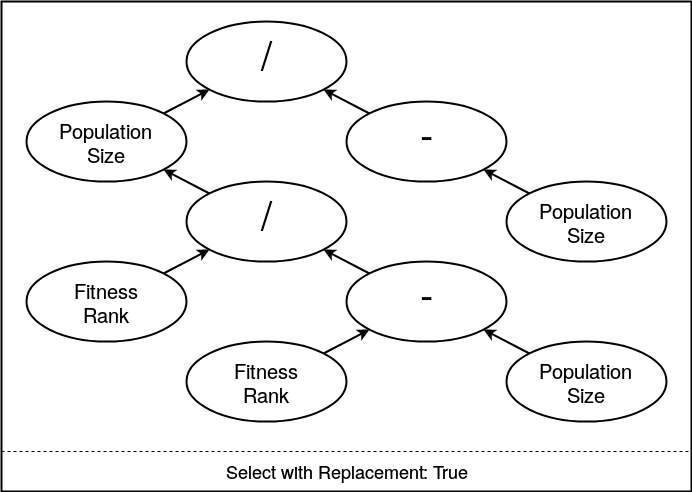
\includegraphics[width=0.475\textwidth]{adpsea_final}
    \caption{One of the best custom selection functions produced by the meta-EA.}
    \label{fig:adpsea_final}
\end{figure}

\section{Discussion}
\label{Discussion}
The results show that the search algorithm found by the meta-EA can outperform several conventional selection algorithms, and that the improved performance of this search algorithm generalizes well to new instances within the same problem class. 

Despite the wide success in generalization of the custom selection function, there were a few testing instances where the custom selection algorithm performed on par with a typical selection algorithm. It is likely that these generated testing instances were simpler landscapes that the typical selection functions were sufficient to find high quality solutions in. It can also be observed, in Figure~\ref{fig:nk_landscape_fitness_boxplot}, that some of the best fitnesses achieved by the typical selection functions are within the interquartile range of the best fitnesses achieved by the evolved selection function. However, the performance increase of the evolved selection function is still statistically significant, to a degree of P<0.001.

When looking at the final best selection algorithm in its GP-Tree form, it is not exactly intuitive what sort of selective strategy it is employing. However, this exemplifies one of the key strengths of Evolutionary Algorithms and Hyper-heuristics, which is that they are unconstrained by human predispositions and biases. With Hyper-heuristics, we can develop new algorithms that are judged purely by their performance, and not necessarily to their conformance to an existing standard or idea.

By examining the trends in fitness of the bottom-level EA using the custom selection algorithm, versus the conventional selection algorithms, it is clear that the custom selection algorithm is better able to promote gradual growth in the fitness of the individuals without getting stuck in a poor local optimum. In some cases, the algorithm even enables the bottom-level EA to converge on a high optimum faster than other selection functions reach a subpar optimum, improving the efficiency of the EA.

One interesting observation is a particular pattern of subtree often observed in the population: a series of Fitness-Rank terminals being multiplied together. The meta-EA likely developed this sequence to introduce a stronger selection pressure than the basic terminals can provide. Intuitively, in a large population, the Fitness-Rank terminal alone does not provide a high selection pressure, as the individual with the second-highest fitness is almost as likely to be selected as the individual with the highest fitness. To achieve a high performance on the benchmark fitness function likely required more selection pressure, especially because the random survival selection scheme provided no selection pressure at all. Multiplying the Fitness-Rank by itself effectively maintains the same order of individuals in the ranking, but with their selection probabilities more spaced out, and thus, when normalized, individuals with higher ranks are relatively more likely to be selected over lower-ranking individuals than they were before. However, this pattern does not appear in all high-performing selection functions, and it did not appear in the final best performing selection function developed by the meta-EA. This suggests that, if the meta-EA did need to increase the selective pressure imposed by the selection function, it had found more than one way of doing so.

\section{Conclusion}
\label{Conclusion}
We hypothesized that a Hyper-heuristic search through the space of selection functions for EAs could improve the performance of an EA on a particular problem class by discovering a specialized selection function. We developed a representation of selection functions that uses a Koza-style GP-Tree to relate an individual's fitness value and fitness ranking to its relative probability of selection, and used a meta-EA to search through the space of selection functions in this representation. After finding a selection function that improved the performance of the EA on the training instances of a problem class, we applied the same EA, with the same selection function, to separate testing instances of the same problem class, and showed the generalization of the performance improvement.

We have shown that, with a meta-EA, it is possible to generate new selection functions, tuned to a particular benchmark problem, that can enable an EA to significantly outperform conventional selection functions on those problems. Thus, we show that, in order to discover the optimum selection method for an EA operating on a particular problem, it is not sufficient to use any of the static conventional selection functions tested. We have also shown that this performance increase from a custom selection algorithm will generalize to similar problems in the same problem class. Therefore, if one expects to run the same EA on many problems from the same problem class, one might expect to gain a performance increase by doing some \textit{a prioiri} calculation to develop a specialized selection algorithm trained on instances of that problem class, which would then enable an EA utilizing that selection function to perform better on all instances of that problem class.

\section{Future Work}
\label{Future Work}

The work presented in this paper opens a number of potential avenues for future research. Of primary concern is the fact that the meta-EA presented in this paper requires a large amount of \textit{a prioiri} computation to generate a high-quality selection function. While this computational cost may be worth it for EAs that will run on problems from the same problem class many times, a more efficient method of finding good selection functions has a much greater potential to benefit EAs in general. 

The NK-Landscape benchmark problem was used as the problem to be solved by the bottom-level EA, and this experiment showed increased performance on that problem class with a specialized, evolved selection function. Future experiments may investigate the performance benefit that can be gained for other problem classes, including real-world problem classes, to more generally explore the practical benefit of specializing selection functions.

Because the objective of this paper is similar to the work done to develop selection algorithms via Grammatical Evolution, it remains to be seen which cases each method is more effective for, and a direct comparison of the two methods on the same benchmark problem may yield more insight into which offers better performance benefits under certain conditions.

The parameters for both the meta-EA and the bottom-level EA were manually tuned for this experiment, and further exploration of optimal parameters, either with software-automated tuning or dynamic adaptation, could improve performance of the EA at both levels. Additionally, both the generated selection functions and the conventional selection functions tested use static parameters throughout the evolution, and more work will be needed to investigate the feasibility of searching the space of more dynamic selection functions.

\bibliographystyle{ACM-Reference-Format}
\bibliography{adpsea-bibliography} 

\end{document}
\grid
\grid
\grid
\grid
\grid
\grid
\grid
